\section{Nonlinear Support Vector Machines}

When applying our SVC to \emph{linearly separable} data in~\eqref{eq:svc_max_wolfe_dual}, we have started by creating a matrix $Q$ from the dot product of our input variables:

\begin{equation} \label{eq:svc_hessian}
	Q_{ij} = y_i y_j k(x_i,x_j)
\end{equation}

or, a matrix $K$ from the dot product of our input variables in the SVR case~\eqref{eq:svr_min_wolfe_dual}:

\begin{equation} \label{eq:svr_hessian}
	K_{ij} = k(x_i,x_j)
\end{equation}

where $k(x_i,x_j)$ is an example of a family of functions called \emph{kernel functions} and:  

\begin{equation} \label{eq:kernel_function}
	k(x_i,x_j) = \langle \phi(x_i), \phi(x_j) \rangle = \phi(x_i)^T \phi(x_j)
\end{equation}

where $\phi(.)$ is the identity function, is known as \emph{linear} kernel.

The reason that this \emph{kernel trick} is useful is that there are many classification/regression problems that are nonlinearly separable/regressable in the \emph{input space}, which might be in a higher dimensionality \emph{feature space} given a suitable mapping $x \rightarrow \phi(x)$.

\subsection{Polynomial kernel}

The \emph{polynomial} kernel is defined as:

\begin{equation} \label{eq:poly_kernel}
	k(x_i,x_j)=(\gamma \langle x_i, x_j\rangle + r)^d
\end{equation}

where $\gamma$ define how far the influence of a single training example reaches (low values meaning ‘far’ and high values meaning ‘close’).

\begin{figure}[h!]
	\centering
	\begin{subfigure}{.49\textwidth}
		\centering
		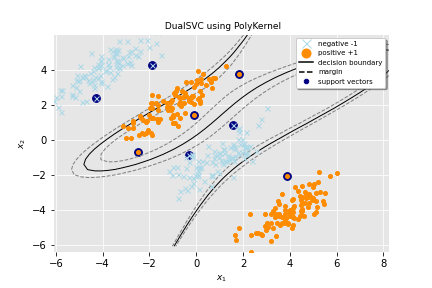
\includegraphics[width=\textwidth]{img/poly_dual_svc_hyperplane}
		\caption{Polynomial SVC hyperplane}
		\label{fig:poly_dual_svc_hyperplane}
	\end{subfigure}
	\begin{subfigure}{.49\textwidth}
		\centering
		\captionsetup{justification=centering}
		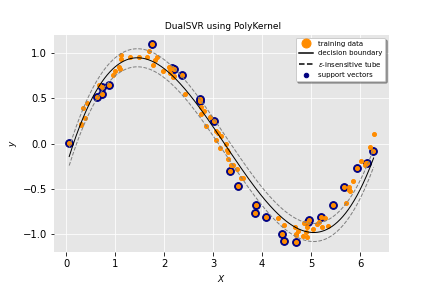
\includegraphics[width=\textwidth]{img/poly_dual_svr_hyperplane}
		\caption{Polynomial SVR hyperplane}
		\label{fig:poly_dual_svr_hyperplane}
	\end{subfigure}
\caption{Polynomial SVM hyperplanes}
\end{figure}

\subsection{Gaussian RBF kernel}

The \emph{gaussian} kernel is defined as:

\begin{equation} \label{eq:gaussian_kernel1}
	k(x_i,x_j)=\exp(-\frac{\|x_i-x_j\|^2}{2\sigma^2})
\end{equation}

or, equivalently:

\begin{equation} \label{eq:gaussian_kernel2}
	k(x_i,x_j)=\exp(-\gamma \|x_i-x_j\|^2)
\end{equation}

where $\displaystyle \gamma=\frac{1}{2\sigma^2}$ define how far the influence of a single training example reaches (low values meaning ‘far’ and high values meaning ‘close’).

\begin{figure}[h!]
	\centering
	\begin{subfigure}{.49\textwidth}
		\centering
		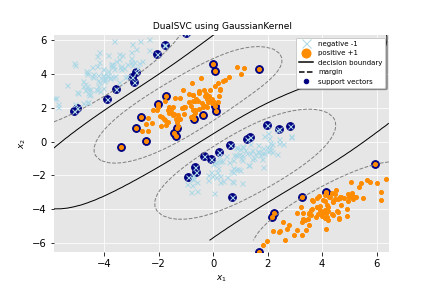
\includegraphics[width=\textwidth]{img/gaussian_dual_svc_hyperplane}
		\caption{Gaussian SVC hyperplane}
		\label{fig:gaussian_dual_svc_hyperplane}
	\end{subfigure}
	\begin{subfigure}{.49\textwidth}
		\centering
		\captionsetup{justification=centering}
		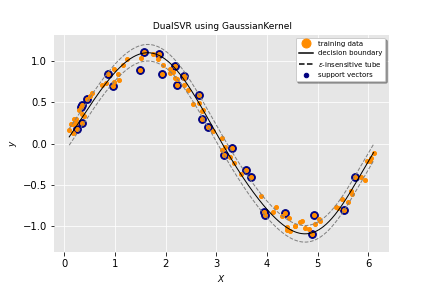
\includegraphics[width=\textwidth]{img/gaussian_dual_svr_hyperplane}
		\caption{Gaussian SVR hyperplane}
		\label{fig:gaussian_dual_svr_hyperplane}
	\end{subfigure}
\caption{Gaussian SVM hyperplanes}
\end{figure}